\documentclass{ctexart}
\usepackage{geometry,amsmath,fancyhdr,lmodern,tikz,graphicx,listings}
\usetikzlibrary{arrows,shapes,chains}
\pagestyle{plain}
\geometry{a4paper,scale=0.8}

\begin{document}

\title{\textbf{实验二~~灰度图像直方图处理}}
\date{}
\maketitle

\paragraph{实验目的:}
\begin{enumerate}
\item 理解和掌握直方图、直方图均衡、直方图匹配的原理和实现方法;
\item 熟悉 matlab 直方图函数、均衡函数的使用;
% \item 实现局域直方图进行图像增强。
\end{enumerate}

\paragraph{实验内容:} 
\begin{enumerate}
\item 直方图均衡化和匹配处理:
\begin{enumerate}
\item 利用 matlab 函数实现图像直方图均衡化处理;显示均衡前后的直方图和图像;
\item 自己编程实现直方图均衡化,并与 matlab 函数的结果进行比较;
\item 自己编程采用直方图匹配的方法重新处理图像,匹配直方图(概率密度函数)自选,
    通过人机交互选择最合适的匹配直方图使图像达到最清晰,可与均衡化的结果进行比较,
    观察匹配结果是否优于均衡结果。
\end{enumerate}
\item 采用局部直方图均衡对图 2.3 进行处理,以获得黑方块内的图像信息。
% \item 对图 2.3 使用直方图统计量局部增强,并与内容 2 中的结果进行比较。
\end{enumerate}

\paragraph{实验原理:} 
\begin{itemize}
\item \textbf{灰度直方图}\\
令$r_k$,k=0,1,2,...,L-1表示一幅L级灰度数字图像f(x,y)的灰度。f的非归一化直方图定义为
\[
    h(r_k)=n_k,~~~~~ k=0,1,2,...,L-1
\]
式中,$n_k$是f中灰度级为$r_k$的像素的数量,并且细分的灰度级称为直方图容器。类似地,f的归一
化直方图定义为
\[
    p(r_k) = \frac{h(r_k)}{MN} = \frac{n_k}{MN}  
\]
式中,M和N分别是图像的函数和列数。多数情况下我们处理的是归一化直方图,我们将这种直方图简单的
称为直方图或图像直方图。\\
暗图像直方图中,大多数直方图容器集中在灰度级的低端;\\
亮图像直方图中,大多数直方图容器集中在灰度级的高端;\\
低对比图像直方图中,大多数直方图容器集中在灰度级的中端;\\
高对比图像直方图中,直方图覆盖较宽范围的灰度级;\\
\item \textbf{灰度直方图均衡化}\\
直方图均衡化是图像处理领域中利用图像直方图对对比度进行调整的方法。\\
连续灰度值的情况下,一幅图像的灰度级可以看成[0,L-1]内的随机变量。随机变量的基
本描绘子是其概率密度函数(PDF)。 r 表示输入图像的灰度值, s 表示均衡化之后的图
像的灰度值, $p_r(r)$ 和 $p_s(s)$ 表示随机变量 r 和 s 的 PDF,因为 r 为输入图像的像素,所
有 $p_r(r)$ 可以求得,则变换之后的 s 的 PDF:
\[
    p_s(s) = p_r(r)|\frac{dr}{ds}|
\]
则有
\[
    s = T(r) = (L-1)\int_0^r P_r(\omega)~d\omega
\]
\[
    \frac{ds}{dr} = \frac{dT(r)}{dr} = (L-1)\frac{d}{dr} [\int_0^r P_r(\omega)~
    d\omega] = (L-1)p_r(r)
\]
\[
    p_s(s) = p_r(r)|\frac{dr}{ds}| = p_r(r)|\frac{1}{(L-1)p_r(r)}| = \frac{1}{L-1},
    ~~0\leq s \leq L-1 
\]
由上式可看出,$p_s(s)$的形式是一个均匀概率密度函数。因此 s 由一个均匀的 PDF 表征。\\
对于离散值,我们用概率与求和来代替概率密度函数与积分。回顾可知,在数字图像中出现灰度级 $r_k$ 
的概率近似为
\[
    p_r(r_k) = \frac{n_k}{MN}
\]
式中,MN是图像中的像素总数,$n_k$ 表示灰度值为 $r_k$ 的像素数。则
\[
    s_k = T(r_k) = (L-1)\sum_{j=0}^k p_r(r_j) = \frac{(L-1)}{MN} \sum_{j=0}^k n_j,
    ~~~~~ k=0,1,2,…,L-1
\]
\item \textbf{灰度直方图规定化}\\
直方图规定化又称为直方图匹配,是指将一幅图像的直方图变成规定形状的直方图而进行的图像
增强方法。即将某幅影像或某一区域的直方图匹配到另一幅影像上。使两幅影像的色调保持一致。\\
设 $P_r(r)$ 和 $P_z(z)$ 分别表示原始灰度图像和目标图像的灰度分布概率密度函数.根据
直方图规定化的特点与要求,应使原始图像的直方图具有 $P_z(z)$ 所表示的形状。根据直方
图均衡化理论,首先对原始图像进行直方图均衡化处理。即求变换函数
\[
    s = T(r) = (L-1) \int_0^r p_r(\omega)d\omega
\]
现假定直方图规定化的目标图像已经实现,因此,对于目标图像也采用同样的方法进行均衡化处
理,因而有
\[
    v = G(z) = (L-1) \int_0^z p_z(t)dt
\]
上式的逆变换为
\[
    z = G^{-1}(v)
\]
上式表明,可通过均衡化后的灰度级v求出目标函数的灰度级z。由于对目标图像和原始图像都进
行了均衡化处理,因此具有相同的分布密度,即
\[
    P_s(s) = P_v(v)
\]
因而可以用原始图像均衡化以后的灰度级s代表v,即
\[
    z = G^{-1}(v) = G^{-1}(s)
\]
所以可以依据原始图像均衡化后的图像的灰度值得到目标图像的灰度级z。\\
对于离散型的灰度,可用下式描述这一过程
\[
    s_k = T(r_k) = (L-1)\sum_{j=0}^k P_r(r_j) = \frac{L-1}{MN} 
    \sum_{j=0}^k n_j, ~~~~~ k = 0,1,2,...,L-1
\]
\[
    s_k = G(\tau_q) = (L-1) \sum_{i=0}^q P_\tau(\tau_i)
\]
\item \textbf{局部灰度直方图}\\
直方图匹配和直方图均匀化的直方图处理方法是全局性的,在某种意义上,像素是被基于整幅图
像灰度满意度的变换函数所修改的,这种全局方法适用整个图像的增强,但有时对图像小区域细
节的局部增强也仍然是适用的。在图像的小区域细节中,像素数在全局变换的计算中可能被忽略,
因为它们没有必要确保局部增强。解决的办法就是在图像中每一个像素的邻域中,根据灰度级分
布(或者其他特性)设计变换函数。该过程定义一个方形或矩形的邻域并把该区域的中心从一像素
移至另一像素。在每个位置的邻域中该点的直方图都要被计算,并且得到的不是直方图均衡化就
是规定化变换函数。这个函数最终被用来映射邻域中心像素的灰度。相邻区域的中心然后被移至
相邻像素位置并重复这个处理过程。其主要原理即为利用直方图均衡化与规定化进行局部增强,
不同点在于操作区域从全局变为一小部分,并且只替换操作中心的灰度值。
\end{itemize}

\paragraph{实验步骤:} 
\begin{itemize}
\item \textbf{实验1:全局灰度直方图的均衡化与规定化}
\begin{itemize}
\item \textbf{使用自带函数实现图像直方图均衡化处理(OpenCV版本)}\\
(1)~使用cv2.imread、cv2.cvtColor函数确保读入灰度图像;\\
(2)~使用cv2.equalizeHist()、cv.calcHist()函数进行灰度图均衡,并绘制直方图;\\
(3)~进行均衡化后图片展示,并展示该图直方图。
\item \textbf{自己编程实现直方图均衡化,并与自带函数结果比较}\\
(1)~计算输入图像的归一化直方图;
\[
    p_r(r_k) = \frac{n_k}{n}, ~~~~~ k = 0,1,2,...,L-1
\]
(2)~计算直方图累进分布函数曲线,直方图均衡化灰度变换函数的离散形式为:
\[
    s_k = T(r_k) = \sum_{j=0}^k p_r(r_j) = \sum_{j=0}^k \frac{n_j}{n},
    ~~~~~ k=0,1,2,…,L-1
\]
(3)~用累积分布函数做变换函数计算图像变换后的灰度级;
\[
    \widehat{s_k} = round[\frac{L-1}{1-s_{min}} (s_k-s_{min})]
\]
(4)~建立输入图像与输出图像灰度级之间的对应关系,变换后灰度级范围应该和原来的范围一致。\\
编程实现框架图如下:\\
\begin{figure}
\scriptsize
\centering
\tikzstyle{startstop} = [rectangle, rounded corners, minimum width = 1cm, minimum height=1cm,text centered, draw = black]
\tikzstyle{process} = [rectangle, minimum width=3cm, minimum height=1cm, text centered, draw=black]
\tikzstyle{decision} = [diamond, aspect = 3, text centered, draw=black]
\tikzstyle{point}=[coordinate,on grid,]
    \begin{tikzpicture}
        \node[process] (one){输入原始图像}; 
        \node[process, right of=one, node distance=4.5cm](two){获得原始图像直方图分布};
        \node[startstop, right of=two, node distance=4.5cm](three){从0到255遍历每一个灰度值};
        \node[process, below of=three, node distance=1.5cm](four){计算每一个灰度值的$S_k$};
        \node[process, below of=four, node distance=1.5cm](five){计算每一个灰度值的非归一化$S(k)$};
        \node[point,right of=five,node distance=3cm](point1){};
        \node[point,right of=three,node distance=3cm](point2){};
        \draw[->] (one)--(two);
        \draw[->] (two)--(three);
        \draw[->] (three)--(four);
        \draw[->] (four)--(five);
        \draw[-](five.east)--(point1);
		\draw[-](point1)-|(point2);
		\draw[->](point2)--(three.east);
    \end{tikzpicture}
\end{figure}

\item \textbf{自己编程实现直方图匹配,人机交互选择合适的匹配直方图}\\
(1)~对$P_r(z)$作直方图均衡化处理,建立输入图像每一灰度级$r_k$与$s_k$的映射关系$r_k \leftrightarrow s_k$:
\[
    s_k = T(r_k) = \sum_{j=0}^k p_r(r_j) = \sum_{j=0}^k \frac{n_j}{n},
    ~~~~~ k=0,1,2,…,L-1
\]
(2)~对$P_z(z)$作直方图均衡化处理,建立输入图像每一灰度级z与v的映射关系z $\leftrightarrow$ v:
\[
    v_q = G(z_q) = \sum_{i=0}^q p_z(z_i), ~~~~~ q=0,1,2,…,L-1
\]
(3)~选择适当的$v_q$与$s_k$点对,使$v_q \cong s_k$;\\
(4)~求G变换的逆变换:
\[
    z = G^{-1}(v) = G^{-1}(s)
\]
(5)~建立的r$\to$z联系,有:
\[
    z = G^{-1}(v) = G^{-1}(s) = G^{-1}(T(r))
\]
编程实现框架图如下:\\
\begin{figure}[htb]
\scriptsize
\centering
\tikzstyle{startstop} = [rectangle, rounded corners, minimum width = 1cm, minimum height=1cm,text centered, draw = black]
\tikzstyle{process} = [rectangle, minimum width=3cm, minimum height=1cm, text centered, draw=black]
\tikzstyle{decision} = [diamond, aspect = 3, text centered, draw=black]
\tikzstyle{point}=[coordinate,on grid,]
    \begin{tikzpicture}
        \node[process] (one){输入原始图像}; 
        \node[process, above of=one, node distance=1.5cm](one_1){输入中心灰度值};
        \node[process, right of=one, node distance=4.5cm](two){获得原始图像直方图分布};
        \node[process,above of=two, node distance=1.5cm](two_2){高斯分布函数获得分布直方图};
        \node[startstop, right of=two, node distance=4.5cm](three){从0到255遍历每一个灰度值};
        \node[process, below of=three, node distance=1.5cm](four){计算每一个灰度值的$S_k$};
        \node[process, below of=four, node distance=1.5cm](five){计算每一个灰度值的非归一化$S(k)$};
        \node[process, right of=five, node distance=4.5cm](six){灰度值与目标高斯分布对应};
        \node[point,right of=five,node distance=2.5cm](point1){};
        \node[point,right of=three,node distance=2.5cm](point2){};
        \node[point,above of=six,node distance=4.5cm](point3){};
        \draw[->] (one)--(two);
        \draw[->] (one_1)--(two_2);
        \draw[-](two_2)--(point3);
		\draw[->](point3)--(six.north);
        \draw[->] (two)--(three);
        \draw[->] (three)--(four);
        \draw[->] (four)--(five);
        \draw[-](five.east)--(point1);
		\draw[-](point1)-|(point2);
		\draw[->](point2)--(three.east);
        \draw[->] (five)--(six);
    \end{tikzpicture}
\end{figure}
\end{itemize} 
\item \textbf{实验2:局部灰度直方图均衡化}\\
(1)~定义一个方形或矩形区域(邻域),该区域的中心位置在某个像素点;\\
(2)~计算该邻域直方图,利用前面介绍的技术得到变换函数;\\
(3)~使用该变换函数来映射该区域的中心像素灰度;\\
(4)~把该区域中心从一个像素移动到另一个像素,重复(2)--(4))。\\
编程实现框架图如下:\\
\begin{figure}[htb]
\scriptsize
\centering
\tikzstyle{startstop} = [rectangle, rounded corners, minimum width = 1cm, minimum height=1cm,text centered, draw = black]
\tikzstyle{process} = [rectangle, minimum width=3cm, minimum height=1cm, text centered, draw=black]
\tikzstyle{decision} = [diamond, aspect = 3, text centered, draw=black]
\tikzstyle{point}=[coordinate,on grid,]
\begin{tikzpicture}
    \node[process] (one){输入原始图像}; 
    \node[process, right of=one, node distance=4.5cm](two){图像矩阵行列扩充};
    \node[process, right of=two, node distance=4.5cm](three){选中中心元素创建邻域};
    \node[process, below of=three, node distance=1.5cm](four){该邻域均衡化};
    \node[process, below of=four, node distance=1.5cm](five){所得结果赋给中心元素};
    \node[decision, below of=five, node distance=1.5cm](six){是否最后一个元素};
    \node[decision, below of=six, node distance=1.5cm](seven){结果是否需再次计算};
    \node[startstop, below of=seven, node distance=1.5cm](eight){输出图像};
    \node[point,right of=six,node distance=3cm](point1){};
    \node[point,right of=three,node distance=3cm](point2){};
    \node[point,left of=seven,node distance=4.5cm](point3){};
    \draw[->] (one)--(two);
    \draw[->] (two)--(three);
    \draw[->] (three)--(four);
    \draw[->] (four)--(five);
    \draw[->] (five)--(six);
    \draw[-](six.east)node[right]{N}--(point1);
    \draw[-](point1)-|(point2);
    \draw[->](point2)--(three.east);
    \draw[->] (six)--node[above]{Y}(seven);
    \draw[-](seven.west)node[left]{Y}--(point3);
    \draw[->](point3)--(two.south);
    \draw[->] (seven)--node[above]{N}(eight);
\end{tikzpicture}
\end{figure}
% \item \textbf{实验3:直方图统计量局部增强}
\end{itemize}

\paragraph{实验结果及代码:} 
\begin{itemize}
\item \textbf{实验1:全局灰度直方图的均衡化与规定化}
\begin{itemize}
\item \textbf{使用自带函数实现图像直方图均衡化处理(Python+OpenCV)}
\lstset{
 columns=fixed,       
 numbers=left,                                        % 在左侧显示行号
 numberstyle=\tiny\color{gray},                       % 设定行号格式
 frame=none,                                          % 不显示背景边框
 backgroundcolor=\color[RGB]{255,255,255},            % 设定背景颜色
 keywordstyle=\color[RGB]{40,40,255},                 % 设定关键字颜色
 numberstyle=\footnotesize\color{darkgray},           
 commentstyle=\it\color[RGB]{0,96,96},                % 设置代码注释的格式
 stringstyle=\rmfamily\slshape\color[RGB]{128,0,0},   % 设置字符串格式
 showstringspaces=false,                              % 不显示字符串中的空格
 language=python,                                        % 设置语言
}
\begin{lstlisting}
# 获取图片
img2_1 = cv.imread("2.1.tif")
img2_1 = cv.cvtColor(img2_1, cv.COLOR_BGR2GRAY)
# opencv直方图均衡
img2_1_dst_cv = cv.equalizeHist(img2_1)
# 绘制直方图
hist2_1 = cv.calcHist([img2_1], [0], None, [256], [0, 256])
hist2_1_dst_cv = cv.calcHist([img2_1_dst_cv], 
                             [0], None, [256], [0, 256])
# 图片展示区域
plt.subplot(3, 2, 1)
plt.imshow(img2_1, cmap='gray')
plt.title('src')
plt.subplot(3, 2, 2)
plt.plot(hist2_1, label="imgSrc", color="b")
plt.subplot(3, 2, 3)
plt.imshow(img2_1_dst_cv, cmap='gray')
plt.title('hist_cv')
plt.subplot(3, 2, 4)
plt.plot(hist2_1_dst_cv, label="imgHist_cv", color="r")
plt.show()
\end{lstlisting}

\item \textbf{自己编程实现直方图均衡化,并与自带函数结果比较(Python+OpenCV)}
\begin{lstlisting}
def hist_equal_my(img):
    # 获取直方图信息
    hist = cv.calcHist([img], [0], None, [256], [0, 256])
    img_dst = img.copy()  # 复制原图获得目标最终图像
    pixels_sum = img.size  # 得到总像素点数
    # 构建中间变量
    img_mid = np.zeros(256)
    img_mid_S_k = np.zeros(256)
    j = 0
    for i in hist:
        # 计算s_k
        if j > 0:
            img_mid[j] = i / pixels_sum + img_mid[j - 1]
        else:
            img_mid[j] = i / pixels_sum
        # 非归一化S(k)
        img_mid_S_k[j] = round(img_mid[j] * 255)
        j = j + 1
    # 图像重映射
    for i in range(img.shape[0]):
        for j in range(img.shape[1]):
            img_dst[i][j] = img_mid_S_k[img[i][j]]
    return img_dst

# 获取图片
img2_1 = cv.imread("2.1.tif")
img2_1 = cv.cvtColor(img2_1, cv.COLOR_BGR2GRAY)
# 自构函数直方图均衡
img2_1_dst_my = hist_equal_my(img2_1)
# 绘制直方图
hist2_1 = cv.calcHist([img2_1], [0], None, [256], [0, 256])
hist2_1_dst_my = cv.calcHist([img2_1_dst_my], 
                             [0], None, [256], [0, 256])
# 图片展示区域
plt.subplot(3, 2, 1)
plt.imshow(img2_1, cmap='gray')
plt.title('src')
plt.subplot(3, 2, 2)
plt.plot(hist2_1, label="imgSrc", color="b")
plt.subplot(3, 2, 5)
plt.imshow(img2_1_dst_my, cmap='gray')
plt.title('hist_my')
plt.subplot(3, 2, 6)
plt.plot(hist2_1_dst_my, label="imgHist_my", color="g")
plt.show()
\end{lstlisting}

\textbf{实验效果图展示如下:}
\begin{figure}[htb]
\centering
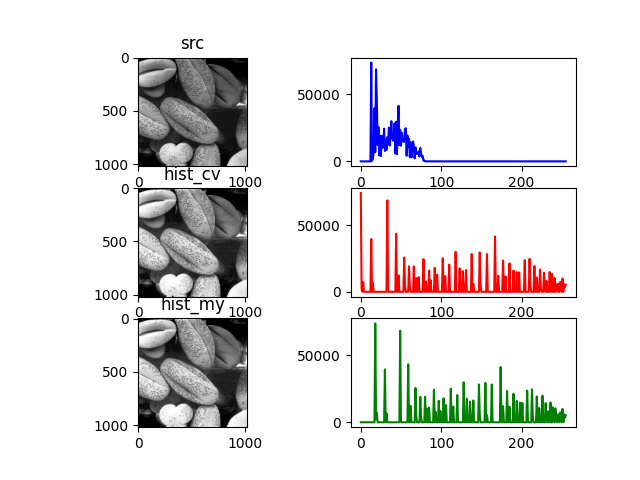
\includegraphics{result.PNG}
\caption{实验1.1与1.2效果图展示}
\end{figure}

\item \textbf{自己编程实现直方图匹配,人机交互选择合适的匹配直方图(Matlab)}
\lstset{
 columns=fixed,       
 numbers=left,                                        % 在左侧显示行号
 numberstyle=\tiny\color{gray},                       % 设定行号格式
 frame=none,                                          % 不显示背景边框
 backgroundcolor=\color[RGB]{255,255,255},            % 设定背景颜色
 keywordstyle=\color[RGB]{40,40,255},                 % 设定关键字颜色
 numberstyle=\footnotesize\color{darkgray},           
 commentstyle=\it\color[RGB]{0,96,96},                % 设置代码注释的格式
 stringstyle=\rmfamily\slshape\color[RGB]{128,0,0},   % 设置字符串格式
 showstringspaces=false,                              % 不显示字符串中的空格
 language=matlab,                                        % 设置语言
}
\begin{lstlisting}
%% Function Match
function [img] = fun_match(a,miu,sigma)
% 直方图匹配函数,miu,sigma输入变量用来生成高斯分布
c=a; % 用来保存原图以作为对比
% 根据高斯函数建立一个概率分布函数
x = 0:1:255;
y0 = 1/(sqrt(2*pi)*sigma)*exp(-(x-miu).^2/(2*sigma^2));

b=sum(y0); % 用来检测概率分布和是否为0
y0=y0/b;  % 使得概率分布函数积分为1
y0=cumsum(y0);
y0=uint8(255.*y0); % y0是想要匹配所得的灰度映射 
cdfa=fun_average(a); % a均衡化的灰度映射

% 将原图灰度映射与新的直方图的映射联系起来,灰度对应
for i=1:256
    %寻找灰度值最近的对应值
    k=min(abs(cdfa(i)-y0));
    for j=1:256
        if abs(cdfa(i)-y0(j))==k
            cdfa(i)=j-1;    % 灰度逆映射
            break
        end
    end
end

% 得到新的从a到y0灰度映射矩阵(从r到z)
% 通过最新映射矩阵将输入图像转化为输出图像
[M,N]=size(a);
for ii=1:M
    for jj=1:N
        a(ii,jj)=cdfa(a(ii,jj)+1);  
    end  
end 
img=a;
end

%% Function average
function [cdfA] = fun_average(A)
[M,N]=size(A);
cdfA=zeros(1,256);

%递增序列统计灰度频数
for i=1:M
    for j=1:N  
    cdfA(A(i,j)+1)=cdfA(A(i,j)+1)+1;  
    end  
end  

%转为频率统计
cdfA=cdfA./(M*N*1.0);
%累积分布函数
cdfA=cumsum(cdfA);  
%将累积分布函数映射到0-255的灰度级
%得到灰度映射向量
cdfA=uint8(255.*cdfA); 
end

%% Main Function
c=imread('2.3.tif');
[a]=fun_match(c,miu1,sigma1); 

[M,N]=size(c);
b=c;%均衡化图
histc=fun_average(c);
for i=1:M
    for j=1:N
        b(i,j)=histc(b(i,j)+1);  
    end  
end
\end{lstlisting}

\textbf{实验效果图展示如下:}
\begin{figure}[htb]
\centering
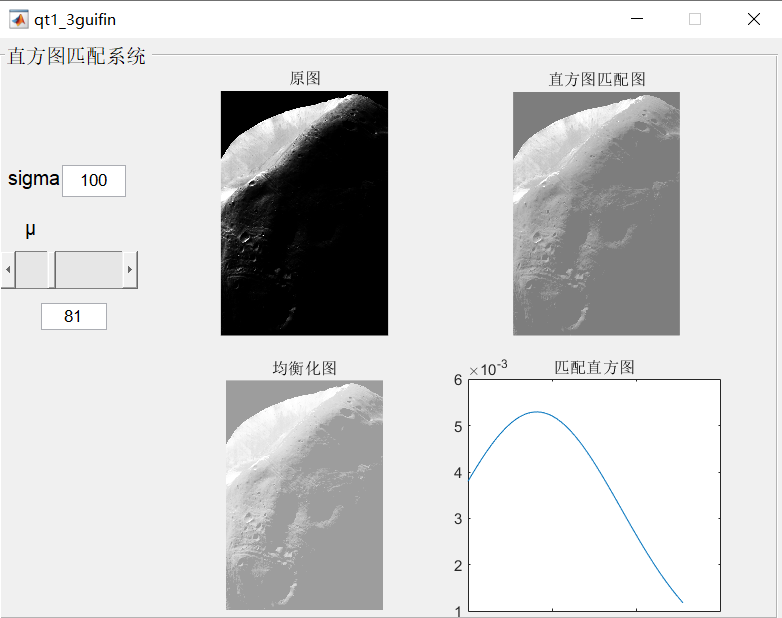
\includegraphics[width=0.5\textwidth]{1_3.png}
\caption{实验1.3效果图展示}
\end{figure}

\end{itemize} 
\item \textbf{实验2:局部灰度直方图均衡化(Matlab)}
\lstset{
 columns=fixed,       
 numbers=left,                                        % 在左侧显示行号
 numberstyle=\tiny\color{gray},                       % 设定行号格式
 frame=none,                                          % 不显示背景边框
 backgroundcolor=\color[RGB]{255,255,255},            % 设定背景颜色
 keywordstyle=\color[RGB]{40,40,255},                 % 设定关键字颜色
 numberstyle=\footnotesize\color{darkgray},           
 commentstyle=\it\color[RGB]{0,96,96},                % 设置代码注释的格式
 stringstyle=\rmfamily\slshape\color[RGB]{128,0,0},   % 设置字符串格式
 showstringspaces=false,                              % 不显示字符串中的空格
 language=matlab,                                     % 设置语言
}
\begin{lstlisting}
A=imread('图2.4.tif');
%对矩阵进行扩展,复制最近边缘值
B=uint8(zeros(258,258));

B(2:257,2:257)=A;
B(1,2:257)=A(1,1:256);
B(258,2:257)=A(256,1:256);
B(2:257,1)=A(1:256,1);
B(2:257,258)=A(1:256,256);
B(1,1)=A(1,1);
B(1,258)=A(1,256);
B(258,1)=A(256,1);
B(258,258)=A(256,256);
C=padarray(A,[2,2],'symmetric');%用函数进行扩展
D=padarray(A,[3,3],'symmetric');%用函数进行扩展,方便对边界值进行赋值

%用3*3邻域进行局部均衡化
for i=2:257
    for j=2:257
        z=B(i-1:i+1,j-1:j+1);
        cdfz=fun_average(z);
        for ii=1:3
            for jj=1:3
                z(ii,jj)=cdfz(z(ii,jj)+1);
            end
        end
        B(i,j)=z(2,2);
    end
end
A_result1=B(2:257,2:257);

%用5*5矩阵邻域局部平衡话
for i=3:258
    for j=3:258
        z=C(i-2:i+2,j-2:j+2);
        cdfz=fun_average(z);
        for ii=1:5
            for jj=1:5
                z(ii,jj)=cdfz(z(ii,jj)+1);
            end
        end
            C(i,j)=z(3,3);
    end
end
A_result2=C(3:258,3:258);

%7*7邻域进行处理
for i=4:259
    for j=4:259
        z=D(i-3:i+3,j-3:j+3);
        cdfz=fun_average(z);
        for ii=1:7
            for jj=1:7
                z(ii,jj)=cdfz(z(ii,jj)+1);
            end
        end
            D(i,j)=z(4,4);
    end
end

A_result3=D(4:259,4:259);
\end{lstlisting}

\textbf{实验效果图展示如下:}
\begin{figure}[htb]
\centering
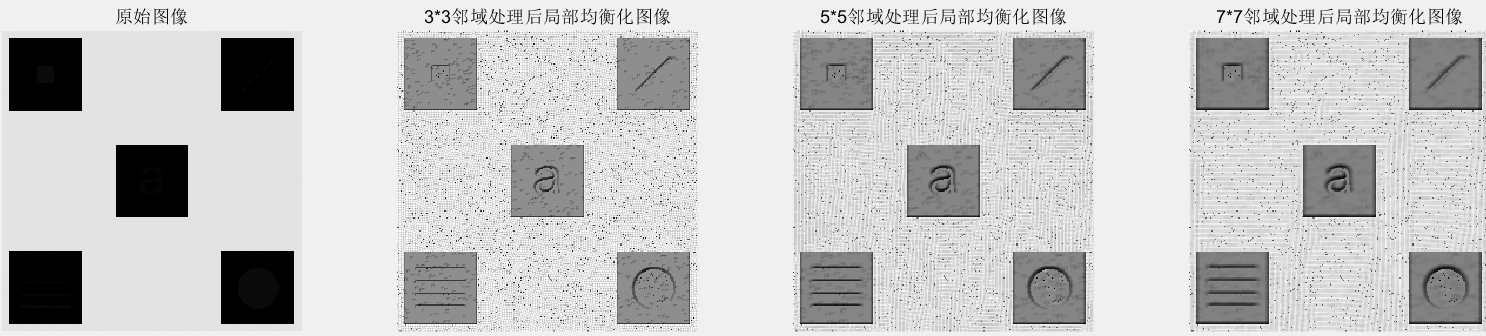
\includegraphics[width=0.95\textwidth]{2_1.png}
\caption{实验2效果图1展示}
\end{figure}

\begin{figure}[htb]
    \centering
    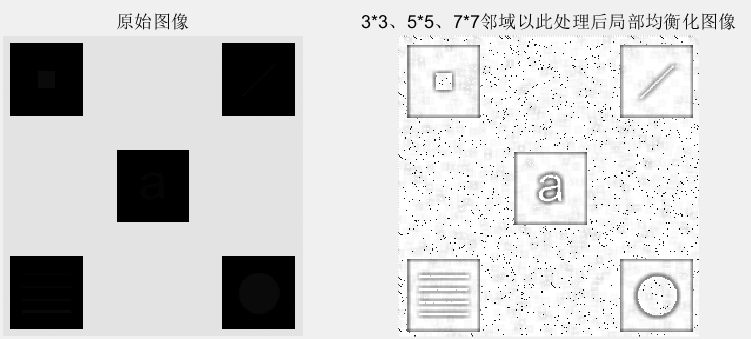
\includegraphics[width=0.5\textwidth]{2_2.png}
    \caption{实验2效果图2展示}
    \end{figure}
% \item \textbf{实验3:直方图统计量局部增强}
\end{itemize}

\paragraph{\textbf{实验结果分析讨论:}} 
\begin{enumerate}
\item \textbf{实验1:全局灰度直方图的均衡化与规定化}\\
1.\textbf{matlab自带函数均衡化}~利用 matlab 函数实现图像的直方图均衡化处理,用到的函数是
$J = histeq(I,n)$,其中I代表原始图像,n代表变换后的灰度级个数。如果想要显示灰度直
方图,可以利用imhist(I)来生成图像的灰度直方图,横坐标是灰度值,纵坐标是某个灰度值
对应的像素点个数。
通过灰度直方图可以看出,原始图像的灰度集中分布在灰度值比较低的区域,而且直方图比较窄,
这说明原始图像是一个低亮度、而且具有较低对比度的图片,其视觉效果并不好。而经过直方图
均衡化之后,其像素占据了很宽的灰度级,并且分布的比较均匀,图片的对比度变得更高。\\
2.\textbf{自己编程实现直方图均衡化,并与 matlab 函数的结果进行比较}~将自编程序处理过的图像和matlab自带函数
histeq处理过的图像进行对比,发现用肉眼难以发现二者的细微区别,直方图的差别也较小,可
以认为自编程序较好的完成了直方图均衡化。\\
3. \textbf{灰度直方图规定化}~,通过选定合适的规定化直方图,发现如果选择合适的直方图进行规定化,
就可以有效地增加图像的对比度,效果可以优于直方图均衡化,但是如果选择的直方图不合适,
其效果就会不如均衡化的图像。所以选取合适的直方图对于直方图规定化来说特别重要。
\item \textbf{实验2:局部灰度直方图均衡化}\\
局部直方图均衡化采用了三种方式,分别是3*3、5*5和7*7邻域处理,可以5*5邻域处理的效果
略好于3*3邻域处理的效果,7*7邻域处理的效果略好于5*5的效果。但之后我们对一幅图像接
连进行重复局部均直方图均衡化处理(即对处理之后的图像再处理),发现效果明显要好于只
使用一次处理之后的直方图,所得图像轮廓更加明显。\\
利用局域直方图的处理可以有效地避免全局均衡化带来的忽略细节的问题,较好的提取出了图片
中某一部分的细节信息。
\end{enumerate}

\paragraph{\textbf{心得体会:}}~\\
在这次实验中,我们学会了直方图的均衡化和规定化,对于全局变量的直方图均衡化算法比较简
单,操作也比较方便;而在直方图规定化的时候,由于需要寻找一个比较适合的规定化直方图,
所以需要进行多次尝试,为此,我们尝试应用了GUI界面,通过手动调节高斯分布函数的参数来
对图像进行快速的调节,可以说这是我们的一个创新点;另一个很有收获的点在局部均衡化处理
的时候发现不同邻域处理累加到一幅图上之后,会取得各种各样的效果,合适的组合会使图像视
觉效果大大增强。

\paragraph{\textbf{实验贡献度:}}~\\
王哲涵 ~~ 35\%\\
岳文杰 ~~ 40\%\\
谢元昊 ~~ 25\%

\end{document}
